\documentclass[french]{article}
 
\usepackage[utf8]{inputenc}
\usepackage[T1]{fontenc}
\usepackage{babel}
\usepackage{advdate}
\usepackage{graphicx} 
\usepackage{amsmath} 
\usepackage{listings}
\usepackage{hyperref}
\usepackage{caption}
\usepackage{subcaption}
\usepackage{listings}

\begin{document}
\begin{titlepage}
\SetDate[29/04/2018]
\newcommand{\HRule}{\rule{\linewidth}{0.5mm}}
\center 
\textsc{\LARGE Université Paris Dauphine}\\[1.5cm] 
\textsc{\Large Data Analytics}\\[0.5cm]
\HRule \\[0.4cm] { \huge \bfseries
Implementation de KMeans avec Spark}\\[0.4cm] \HRule \\[1.5cm]
\begin{minipage}{0.4\textwidth}
	\begin{flushleft} \large
		\emph{Etudiants}
		\\ Elie \textsc{Abi Hanna Daher}
		\\ Bilal \textsc{El Chami}
		\\ Badr \textsc{Erraji}
	\end{flushleft}
\end{minipage}
~
\begin{minipage}{0.4\textwidth}
	\begin{flushright} \large
		\emph{Professeur} 
		\\ M. Benjamin \textsc{Negrevergne}
		\\  \hspace{1cm}
		\\  \hspace{1cm}
	\end{flushright}
\end{minipage}\\[2cm]
{\large \today}\\[2cm]

\includegraphics[width=8cm]{img/dauphine.png}
\vfill
\end{titlepage}
 
\tableofcontents 
\newpage
La méthode K-means est une des méthodes de clustering les plus utilisée lors de l’implémentation d’algorithmes cherchant à grouper un ensemble de données disparates. Cette méthode repose principalement sur le \textit{unspervised learning}.
L’objectif étant alors de grouper ces dernières en 'implémenté l'algorithme KMean avec Spark (python) et en évaluant la performance de notre implémentation basé sur des données que nous générons.

\section{Travail effectué}
\subsection{Implementation}
\subsubsection{Kmeans}
\subsubsection{Generateur}
Afin d’évaluer l’algorithme KMeans implémenté, un générateur de données est mis en place. \\

On a mis en place 2 fichier de python : \textit{generator.py} et \textit{generator-noise.py} \\
Le fichier \textit{generator.py} permet de générer des points et de les sauvegarder dans un fichier. \\
Le deuxième fichier, \textit{generator-noise.py}, permet de générer les points ainsi qu’il génère des points bruits qui sont générer aléatoirement.\\

Afin de sauvegarder les données dans un fichier externe, on a implémenté 2 façons différentes : 
\begin{itemize}
\item 	\textit{saveAsTextFile} : qui est une méthode déja présente qui sauvegarde un rdd
\item 	\textit{write-into-csv} qui est une méthode que nous avons créer qui permet d'écrire directement dans un fichier les valeurs du RDD
\end{itemize}
La méthode que nous avons créer, \textit{write-into-csv},  permet de generer un seul fichier mais n'est pas efficient et ne profite pas des caractéristiques du RDD c'est pour cela la méthode saveAsTextFile est meilleur en terme d'efficacité. Cette derniere créer plusieurs fichiers.

\begin{figure}[h!]
\centering
\begin{subfigure}{.5\textwidth}
  \centering
  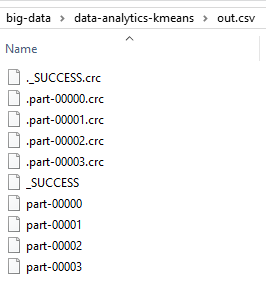
\includegraphics[width=.4\linewidth]{img/save-text-file.png}
  \caption{Méthode \textit{saveAsTextFile}}
  \label{fig:sub1}
\end{subfigure}%
\begin{subfigure}{.5\textwidth}
  \centering
  
\includegraphics[width=.4\linewidth]{img/write-into-csv.png}
  \caption{Méthode \textit{write-into-csv}}
  \label{fig:sub2}
\end{subfigure}
\caption{Fichier output de chaque méthode du générateur de données}
\label{fig:test}
\end{figure}

\newpage
\noindent En exécutant, le \textit{generator.py} avec la commande suivantes : 
\begin{lstlisting}[language=bash]
  $ spark-submit generator.py out 9 3 2 10
\end{lstlisting}
Les points sont générés, et en affichant les résultats dans le graphique on obtient :
\begin{figure}[h!]
  \centering
  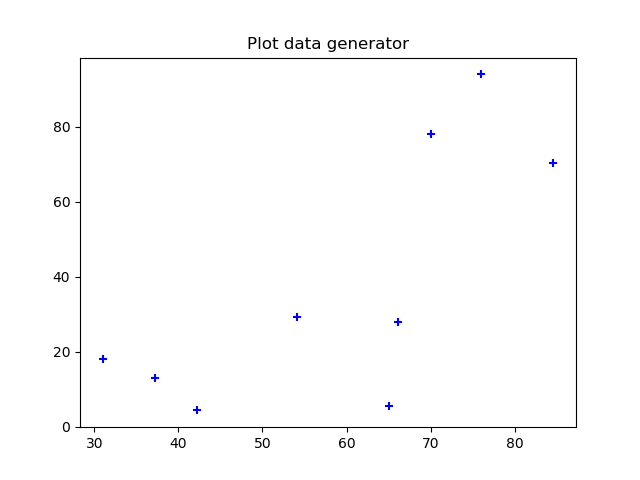
\includegraphics[width=\linewidth]{img/generator-points.png}
  \caption{Generateur des points}
\end{figure}


\noindent En executant, le \textit{generator-noise.py} avec la commande suivantes : 
\begin{lstlisting}[language=bash]
  $ spark-submit generator_noise.py out 9 3 2 10
\end{lstlisting}
Le nombre de bruits est le double du nombre des points à générer. 
Les points sont générés, et en affichant les resultats dans le graphique on obtient :
\begin{figure}[h!]
  \centering
  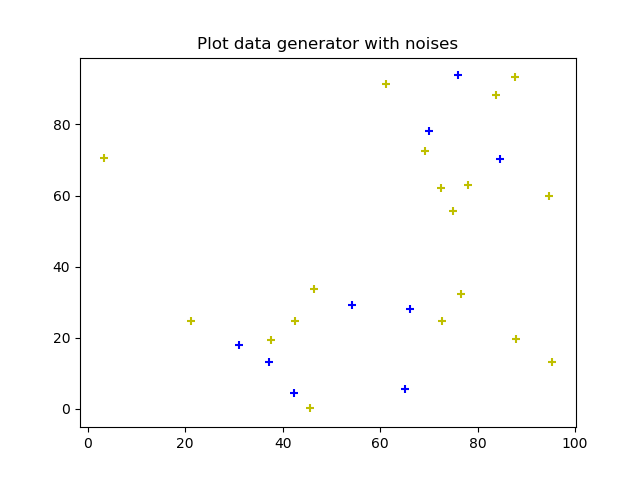
\includegraphics[width=\linewidth]{img/generator-noises.png}
  \caption{Generateur des points avec des bruits}
\end{figure}

\newpage
\subsubsection{Plot}
Afin de générer les graphiques, nous avons utilisés la librairies \textit{matplotlib.pyplot}.\\
Pour les fichiers kmeansPlusPlus, Kmeans nous avons créer 2 fichiers pour chacun, 1 sans plot et 1 avec plot.

Pour chaque itérations, une image est sauvegarder dans le répertoire afin d'analyser l'evolution du résultat.

Les graphes générer sont de 2 dimensions, ce qui indique que si les points ont plus de 2 coordonnées ca ne seras pas tres bien representé graphiquement.
Afin de voire des exemples d'execution, veuiller voir la section Simulation.

\newpage
\subsection{Simulation}
\subsubsection{Kmeans}

\noindent En exécutant, le \textit{kmeans-plot.py} avec la commande suivantes : 
\begin{lstlisting}[language=bash]
  $ spark-submit kmeans-plot.py data/iris-small.dat 3 10
\end{lstlisting}

Le graphe suivant représente les résultats de la premirer iteration et en affichant les 2 premiers coordonnées : sepal width et sepal height
\begin{figure}[h!]
  \centering
  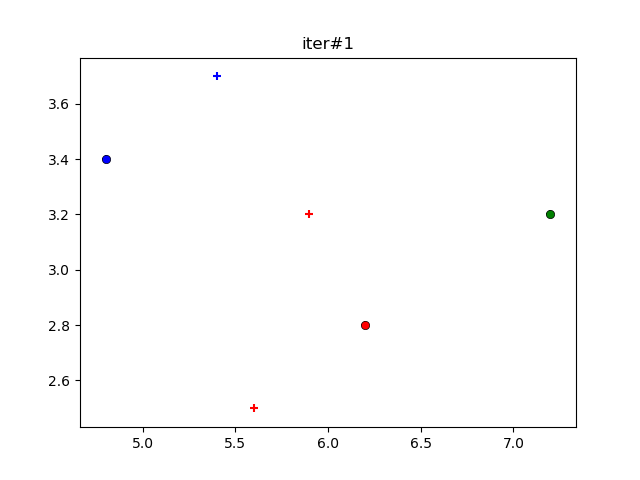
\includegraphics[width=\linewidth]{img/result-kmeans-1.png}
  \caption{Iteration 1}
\end{figure}

Pour trouver le resultat final on a eu besoin de 2 iterations avec une distance finale de $0.9711$ d'ou le resultat final est le suivant
\begin{figure}[h!]
  \centering
  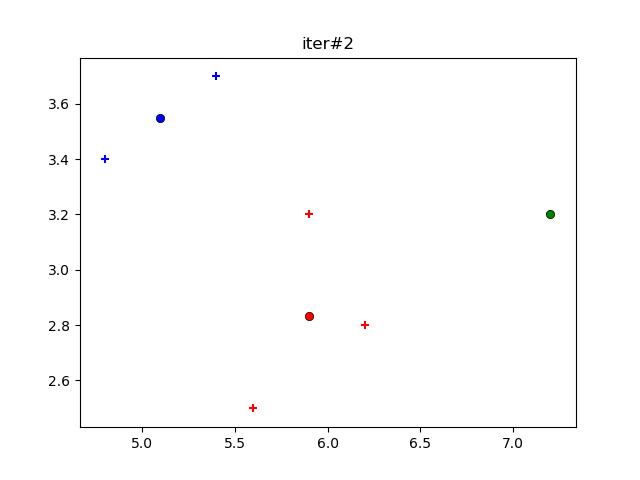
\includegraphics[width=\linewidth]{img/result-kmeans-final.png}
  \caption{Iteration finale}
\end{figure}

Et sur la console on obtient le résultat suivant : 
\begin{figure}[h!]
  \centering
  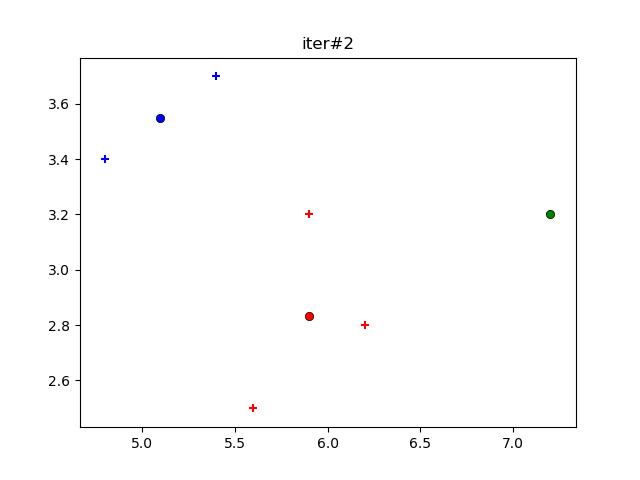
\includegraphics[width=\linewidth]{img/result-kmeans-final.png}
  \caption{Console}
\end{figure}

\newpage
\subsubsection{Executions}
    \begin{table}[!hbt]
        \begin{center}
        \caption{ 100 executions }
        \label{tab:simParameters}
        \begin{tabular}{|c|c|}
            \hline
           Algorithme & distance intra-cluster   \\
            \hline
           KMeans - implémenté & $0.02$  \\
            \hline
           KMeans++ - implémenté & $0.02$ \\
            \hline      
           KMeans & $0.02$ \\
            \hline
        \end{tabular}
        \end{center}
    \end{table}

\section{Analyse}


\section{Application}

\newpage
\begin{thebibliography}{5}
    \bibitem{MonteCarloKakuro} 
    T.~Cazenave. {\em Monte-Carlo Kakuro}
   \bibitem{WikiKakuro} 
   Wikipedia page on {\em Kakuro}. [Online]. \\ Available:  \url{ https://en.wikipedia.org/wiki/Kakuro}
   \bibitem{WikiCSP} 
   Wikipedia page on {\em CSP }. [Online]. \\ Available:  \url{https://en.wikipedia.org/wiki/Constraint_satisfaction_problem}
   \bibitem{WikiBacktracking} 
   Wikipedia page on {\em Backtracking algorithm}. [Online]. \\ Available:  \url{https://en.wikipedia.org/wiki/Look-ahead_(backtracking)}
\end{thebibliography}
\end{document}